\renewcommand{\footerfilename}{QuickCrib.tex}

\section{Quick Crib}  \label{sec:QuickCrib}
% /home/git/external/BonMots/tex/BonMots/QuickCrib.tex

A collection of handy things to know right off the bat:
\vspace{-.15cm}
\begin{enumerate}\addtolength{\itemsep}{-0.5\baselineskip}
%\setcounter{enumi}{N}
   \item   IRAF stands for ``Image Reduction and Analysis Facility''.
   \item   \dhl{AT NO TIME USE UNICODE CHARACTERS}. IRAF is strictly \dhl{ASCII}.
   \item   Three main tasks \textbf{\emph{cl}}, \textbf{\emph{ecl}} and \textbf{\emph{PyRAF}}.
   \item   \textbf{\emph{To exit}} \dhl{cl} or \dhl{ecl} type \dhl{logout} at the prompt.\index{exiting!cl/ecl}
   \item   \textbf{\emph{To exit}} \dhl{PyRAF} use \dhl{.ex} at the prompt.\index{exiting!pyraf}
   \item   \textbf{\emph{To exit}} \dhl{bash} use \dhl{exit} at the prompt.\index{exiting!bash}
   \item   \textbf{\emph{IRAF uses WEST LONGITUDE}}.
\end{enumerate}

\subsection{Commands}

\vspace{-.15cm}
\begin{enumerate}\addtolength{\itemsep}{-0.5\baselineskip}
   \item   IRAF consists of \textbf{\emph{Packages}} that use \textbf{\emph{tasks}} (not \dhl{commands} in usual sense).
\vspace{-.15cm}
    \begin{enumerate}\addtolength{\itemsep}{-0.5\baselineskip}
         \item   Tasks are in \dhl{packages}.
         \item   Both \dhl{packages} and \dhl{tasks} have parameters.
    \end{enumerate}
   \item   IRAF parameters are \dhl{sticky}, the new values persist across sessions!
\vspace{-.15cm}
\begin{enumerate}\addtolength{\itemsep}{-0.5\baselineskip}
%\setcounter{enumi}{N}
   \item   The \dhl{unlearn <taskname>} resets to defaults.
\end{enumerate}

   \item   IRAF tasks use switch characters '+' and '-' that appear at the \textbf{\emph{end of the word}}.
   \item   IRAF's uses the \dhl{epar} GUI where you may set the myrid of variables for a task.
   \item   IRAF uses Unix Commands (ls, mkdir etc):
\vspace{-.15cm}
\begin{enumerate}\addtolength{\itemsep}{-0.5\baselineskip}
%\setcounter{enumi}{N}
   \item   None are built in, but are declared as \dhl{foreign}. You can add to \gls{foreign} commands.
   \item   Non-foreign commands can be run by \dhl{escaping} to the shell. Use the exclamation point \llbox{!}
   to run plain Unix commands in a \dhl{sub-shell}. EG: string the commands \dhl{sed | sort | uniq} together
   for special results.
\end{enumerate}
   \item   Standard IRAF commands are built in.
   \item   Commands can be run as their python functional equivalents:
\end{enumerate}

\newpage
\subsection{IRAF/PyRAF Help} \label{sec:IRAF_PYRAF_Help}

At a command prompt enter:\\
   \verb=--> help =

You can use {\color{verbcolor}\verb/help help dev=ps/} to get a .ps file of the output. Convert this
to PDF using traditional ways.

\subsection{Programs are called Tasks}

Tasks are grouped in a \gls{package}. Packages allow a small subset of
tasks to be loaded into memory at a time. This comes from the days of
small memory capacity on computers at the time IRAF was created.

Each \gls{task} usually has a set of \gls{parameters} where variables
that define its operation are set and maintained.

Tasks are ``\dhl{sticky}'' \index{sticky}. The parameters persist over class. This is a nuisance 
when two instruments are reduced using the same package. To reset a task, use
the unlearn command.

\subsection{FITS Files}

FITS stands for ``Flexible Image Transport System'' It is ``fits'' not ``fit''.

Most files are a ``\dhl{single extension file}''. There is only one section with
a data array. However! FITS permits ``\dhl{multiple extension files}'' or MEFs.
The \dhl{combine} tasks will add an extension each time they are run, and following
commands like imarith will experience an error when trying to operate with one
file as a MEF. 

\textbf{\emph{\color{verbcolor}{Takeaway} :}~ }
Therefore, each time you \dhl{remake} a zero/dark/flat master, remember
to \dhl{remove} the old one first.

\subsection{IRAF/PyRAF Graphics Window}

Exiting graphical tasks can be tricky: \index{exiting!tasks}

\vspace{-.15cm}
\begin{enumerate}\addtolength{\itemsep}{-0.5\baselineskip}
%\setcounter{enumi}{N}
   \item   The \llbox{Q} or \llbox{q}  will usually get you back into a scripts normal way of doing
  things.
   \item   In theory the capital \llbox{I} will interrupt. Not all subtasks will see this.
   \item If you are really stuck use \mousebox{Ctrl-Z} to pause the
     task, dropping back into \dhl{bash}, then kill PyRAF session with
     a:
\begingroup \fontsize{10pt}{10pt} \selectfont
\begin{verbatim} 
    jobs            # list the current tasks for this window
    kill %<n>       # using the job number above

or in a real pinch:

    ps aux | grep -i pyraf   # get the pid (see man ps)
    kill -9 <pid>
\end{verbatim}
\endgroup
   \item   Bite the bullet and ``yes/no'' your way out of trouble.
\end{enumerate}

\subsection{Output from IRAF/PyRAF Tasks}

An optional \dhl{logfile} is associated with important tasks. You can set the name,
or take the default.

When the spectrographic task \dhl{apall} is run, a directory called
\dhl{database} is created. Each file records the details of the extraction
(specifically the conditions/coefficients of polynomials) in a file
whose name is along the lines of ap<filename> (``ap'' prepended to the
filename). The last file is duplicated with aplast.

In the graphics window, a little plus sign at the bottom/left allows
a small text display area to show details of tasks. This is handy in tasks
like \dhl{splot}.

\begin{figure}[h!]
\centering
%%\phantomsection
%%\addcontentsline{toc}{section}{}
%%\caption{} %% \caption{{\tiny{citation}}} 
%%\includepdf[angle=90,width=.3\textwidth]{}); %% with package pdfpages
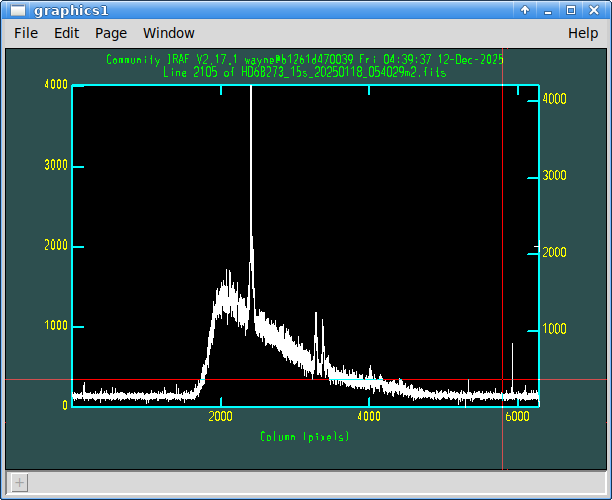
\includegraphics[width=.3\textwidth]{images/pyraf1.png}
\caption{Little ``+'' sign in bottom/left hand corner.} %% \caption{{\tiny{citation}}} 
\label{figure:}
\end{figure}

\subsection{File Names}

Unix and IRAF/PyRAF \dhl{parse} command lines by breaking the line into parts
using spaces.\\
 \textbf{\emph{NOTE}}: \dhl{BREAK THE HABIT PUTTING OF SPACES IN FILENAMES}.

Avoid using spaces, plus/minus signs, punctuation (ampersand,
asterisks, colons and semicolons in particular, sharp character), and
other non [A-Za-z0-9]. Always start a filename with a letter. Keep the
names as short as possible.

\textbf{Trick:} prepend a single letter and underscore (z\_ for zero subtracted files for
example). This is easily done and discussed herein.

\subsection{Lists of Filenames (@lists)}

IRAF uses ``\dhl{list files}'' \index{"@!list files}. This is a filename with an ``at cost'' (@) sign prepended to
the file's name. The file consists of one filename per line and tasks will iterate the
action of each of the files in turn.

Hint: Use ``l.l'' as the list file's name. 

\example Make my zeromaster file and subtract that file from the non-zero files in the directory.


\exercise. I create a zeromaster, being careful not to do the step with a previous zerocombine
file, then for non-zero files, subtract that master. Whew a few steps!

\prose Type the lines into my reduce.pyraf file first, then execute. 

\begingroup \fontsize{10pt}{10pt}
\selectfont
\begin{verbatim} 
--> !ls -1 *zero*.fits > l.l
--> cat l.l
--> hedit @l.l IMAGETYP zero add+ update+ del- ver- show-
--> !rm -f zeromaster.fits   # remove the existing master first.
--> zerocombine @l.l output=zeromaster.fits combine=average scale=none
--> !ls -1 *fits | grep -vi zero > l.l   # get rest of the files
--> imarith @l.l - zeromaster.fits z_@l.l
\end{verbatim}
\endgroup

\takeaway Hope I named the zero files, with a zero in the
filename. Let Unix do its thing, make a l.l list. Then cat l.l
(remember I always check my work) to make sure the list is indeed the
files I want to mangle. Then add IMAGETYP of 'zero' to each of those
files, needed by default setting in the zerocombine step.  To be sure
use \dhl{!rm -f zeromaste.fits} (the -f unix switch will not fail if
the file is not there to begin with); Now combine all the files in the
list into one master file. Now get a list of all the other files (same
dimensions or shape) that ARE NOT ZERO files into my next list file
(\dhl{grep -vi zero} says to omit files matching 'zero'). The imarith
step subtracts the zeromaster.fits (acting as a scalar) from each of
the files in the \dhl{l.l} list with the output going into z\_filename.fits.
Now I have the orignial files and one with z\_ prepended!
Cut past from reduce.pyraf file one line at a time and watch the
progress of the steps to assure nothing untoward has happened.


\subsection{Directories: Location and Naming}

For observations: create a desktop link (shortcut) of
\dhl{\textasciitilde{}/Desktop/Today} folder, and initialize all the
acquisition software to save files into that directory. At the end of
the night simply rename/move the directory to your prefered location
and immediately create a new \dhl{\textasciitilde{}/Desktop/Today}
folder. \dhl{Hint}: means several packages are configured once, and may
be quickly deployed when taking data.


\subsection{Using IRAF Tasks in PyRAF}

The task \dhl{images.imutil.imstatistics} or \dhl{imstat} allows for a
reduced number of fields to be listed.
Note: Using \dhl{Stdout=1} returns a python list, so we capture that.


\example How do we use IRAF routines as python functions, capture output etc.

\prose Hey, I just want to subtract the average mean (haha) of my raw zero exposure files from
from my files. What is that value? I need a list of the mean from each file, then use 
numpy to get the mean and std of that list.

\exercise Write a few snippets of code to prove to myself this will work.

\begingroup \fontsize{10pt}{10pt}
\selectfont
%%\begin{Verbatim} [commandchars=\\\{\}]
\begin{verbatim} 
--> means = list(map(float, iraf.imstat(images='Flat*', format=iraf.no, fields='mean', Stdout=1)))
\end{verbatim}
\endgroup
%% \end{Verbatim}

Unwind this statement: At the core is the command \dhl{iraf.imstat}, with parameters:

\begingroup \fontsize{10pt}{10pt}
\selectfont
%%\begin{Verbatim} [commandchars=\\\{\}]
\begin{verbatim} 
--> mymeans = iraf.imstat(images='Zero*', format=iraf.no, fields='mean', Stdout=1)
\end{verbatim}
\endgroup
%% \end{Verbatim}

\begin{quote}
Indicating to use images \dhl{Zero*} as input; use
\dhl{format=iraf.no} to suppress the printout column header; use
\dhl{fields='mean'} to only get the mean using the imstatistics
algorithm; and have python send the output as a list.
\end{quote}


The \dhl{mymeans} 'list' is in ASCII representation of floats
surrounded by whitespace. The python \dhl{float()} will tolerate appropriate
whitespace. Lets use python's map function. This returns an list BUT WRAPPED
inside a pythonic iterator.

\begingroup \fontsize{10pt}{10pt}
\selectfont
%%\begin{Verbatim} [commandchars=\\\{\}]
\begin{verbatim} 
(map(float,mymeans))  # apply float to each of list's values, returns iterator
\end{verbatim}
\endgroup
%% \end{Verbatim}

But we want a plain python \dhl{list}. So we have to convert the iterator back to
a list:
\begingroup \fontsize{10pt}{10pt}
\selectfont
%%\begin{Verbatim} [commandchars=\\\{\}]
\begin{verbatim} 
list((map(float,mymeans))
# or all together...
mymeans = list(map(float, iraf.imstat(images='Flat*', format=iraf.no, fields='mean', Stdout=1)))
   [1425.136, 1425.099, 1425.024, 1425.829, 1425.7, 1425.645, 
    1425.543, 1425.49, 1425.424, 1425.201, 1425.188]  # formated here for article
# list them:
mymeans
#   [1425.136, 1425.099, 1425.024, 1425.829, 1425.7, 1425.645, 
#    1425.543, 1425.49, 1425.424, 1425.201, 1425.188]  # formated here for article
\end{verbatim}
\endgroup
%% \end{Verbatim}

Here are the parameters for imstatistics:
\begingroup \fontsize{10pt}{10pt}
\selectfont
%%\begin{Verbatim} [commandchars=\\\{\}]
\begin{verbatim} 
      (images = ""              List of input images
      (fields = "image,npix,mean,stddev,min,max") Fields to be printed
       (lower = INDEF)          Lower limit for pixel values
       (upper = INDEF)          Upper limit for pixel values
       (nclip = 0)              Number of clipping iterations
      (lsigma = 3.0)            Lower side clipping factor in sigma
      (usigma = 3.0)            Upper side clipping factor in sigma
    (binwidth = 0.1)            Bin width of histogram in sigma
      (format = yes)            Format output and print column labels ?
       (cache = no)             Cache image in memory ?
        (mode = "al")  
\end{verbatim}
\endgroup
%% \end{Verbatim}

\subsection{Graphics Window}

Sometimes the graphics window can become stuck. Try the key sequence \\
\llbox{l} and \llbox{r}\\
in quick succession.
